\section{Study Frameworks}
    To comprehensively describe the approach that this study takes, this chapter illustrates and explains the frameworks that this study follows. The frameworks show the flow of logic and processes behind this study that allows the study to meet its objectives.
\subsection{Theoretical Framework}

The theoretical framework illustrates the different theories involved in this study and how they relate to each other in order to achieve the study's objective. Figure \ref{fig:theoretical-framework} below shows this study's theoretical framework.
\begin{figure}[H]
    \centering
    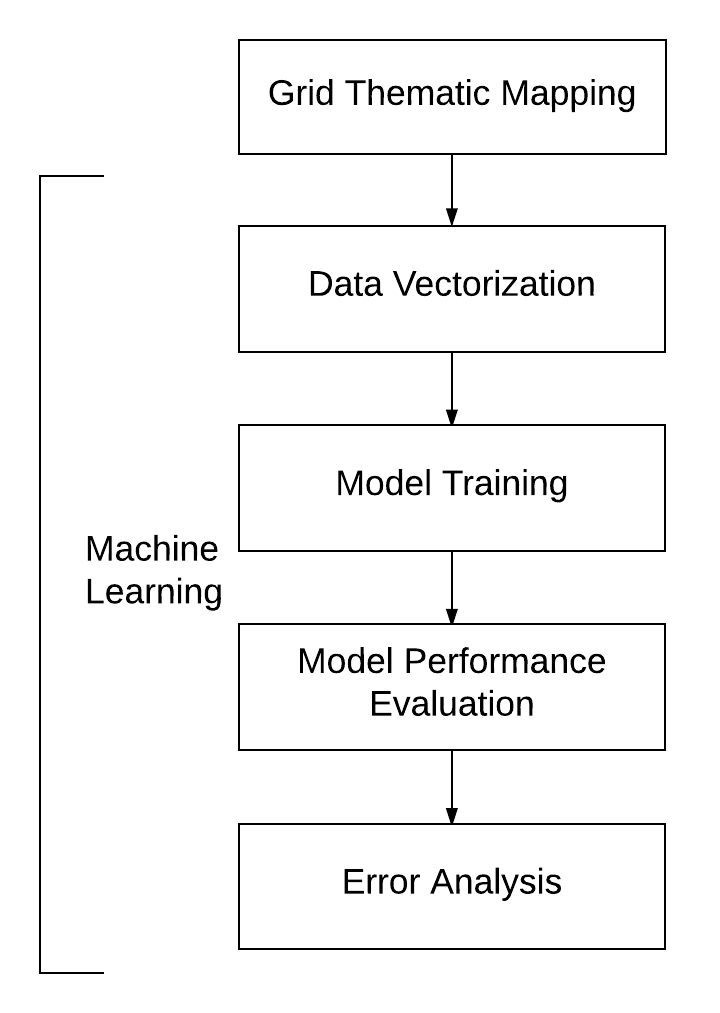
\includegraphics[width=7cm]{theoretical-framework}
    \caption{The theoretical framework of the study}
    \label{fig:theoretical-framework}
\end{figure}
In order to map crimes, we need a way to generate hotspots \cite{eck2005mapping}. By generating possible hotspots, we can easily analyze crimes and map them. One of the easiest and fastest way to identify hotspots is grid thematic mapping \cite{chainey2008utility}. Grid thematic mapping is done through placing uniform cells over a geographical area and thematically shading them. Problems involving different shapes and dimensions of geographical areas can be addressed and dealing with consistent dimensions allows easier and quicker analysis and comparison.

After generating the grid, we can commence machine learning. Machine learning is the study and computer modeling of learning processes and algorithms \cite{michalski2013machine}. In the case of this study, crime hotspots is learned and predicted through a model employing the algorithm of Recurrent Neural Network (RNN) with Long Short-term Memory (LSTM) architecture. 

Machine learning starts by generating our data vectors. Meaningful data is extracted from the information expressed by the presence and absence of criminal records in the different cells generated through grid thematic mapping.

The LSTM model is then trained with this data in order to learn the nature of crime with respect to the cells in the grid. The LSTM network learns by storing data representation of previous input events in forms of activation embodied by the weighted connections between gates and inputs/outputs \cite{hochreiter1997long}. It processes data using the following set of functions as described by Graves \cite{graves2013generating} and as illustrated and explained in Section 2.6 of this paper. The output \( h_t \) of the LSTM layer at timestep $t$ is the function of the input for the input \( x_t \) and the output \( h_{t-1} \) and cell state \( C_{t-1} \) of the layer from the previous timestep by:
    \begin{align}
    i_t &= \sigma(x_t W_{xi} + h_{t-1} W_{hi} + C_{t-1} W_{Ci} + b_i) \label{eq:input}\\
    f_t &= \sigma(x_t W_{xf} + h_{t-1} W_{hf} + C_{t-1} W_{Cf} + b_f) \label{eq:forget}\\
    C_t &= f_t C_{t-1} + i_t \tanh(x_t W_{xC} + h_{t-1} W_{hC} + b_C) \label{eq:cell}\\
    o_t &= \sigma(x_t W_{xo} + h_{t-1} W_{ho} + C_t W_{Co} + b_o) \label{eq:output} \\
    h_t &= o_t \tanh(C_t) \label{eq:h}
    \end{align}

The three gates of an LSTM, namely the input \( i_t \), forget \( f_t \) and output \( o_t \) gates are activated for the current timestep $t$ using the Equations \ref{eq:input}, \ref{eq:forget} and \ref{eq:output} respectively. The cell state for the layer \( C_t \) is updated using Equation \ref{eq:cell}. Finally, the output for the current layer \( h_t \) is produced by Equation \ref{eq:h}. The value \(W_{ab}\) is the weighted connection between $a$ and $b$ so \(W_{xC}\), for instance, denotes the weighted connection between the input node of the current layer and the cell state. The LSTM network goes through all the inputs and outputs and adjusts its weight matrix, or the different values of $W$, accordingly. The final model is a set of weight matrix that is applied to future inputs to predict outputs.

After training, the LSTM model must undergo tests and experiments as part of machine learning in order to assess its performance. It is important to measure the accuracy and precision of the model in order to evaluate if it performed well or not. To understand why it performed as such, error analysis is also done.

Error analysis is done to the model in order to understand its performance and determine further steps to improve the model. To analyze the error, learning curves are generated. A learning curve shows the training error and validation error of the model for different number of training sizes. It helps determine if the model suffered from a high-bias or high-variance.
\begin{figure}[H]
    \centering
    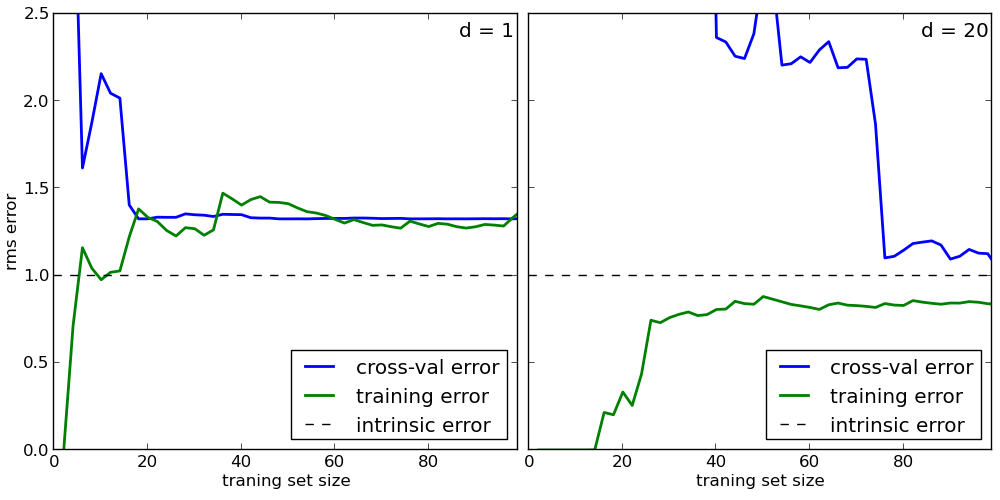
\includegraphics[width=8cm]{plot-bias-variance-examples}
    \caption{Learning curves showing high-bias(left) and high-variance(right) \cite{scikit-learn}}
    \label{fig:learning-curve-sample}
\end{figure}

Figure \ref{fig:learning-curve-sample} shows an example of learning curves of models suffering from high-bias and high-variance. In the left graph, both error curves are very high and overlap each other. This is a case of high-bias error or underfitting. The model fails to achieve a generalization for the set of training examples. To solve underfitting, it will help to add more features so that the model have more parameters to learn from and therefore achieve generalizations better. On the other hand, the right graph shows a case of high-variance error or overfitting. It is characterized by the convergence of the training error and the validation error to a relatively low value while maintaining a large gap in between. The model, in this case, over-generalized the training examples that it fails to predict the correct outputs during validation. To solve this problem, the model should use fewer or simpler features and use more training examples to avoid over-generalizing the data.

\subsection{Conceptual Framework}
The conceptual framework illustrates the application of the theories specific for the study through concepts. Figure \ref{fig:conceptual-framework} shows this study's conceptual framework.
\begin{figure}[H]
    \centering
    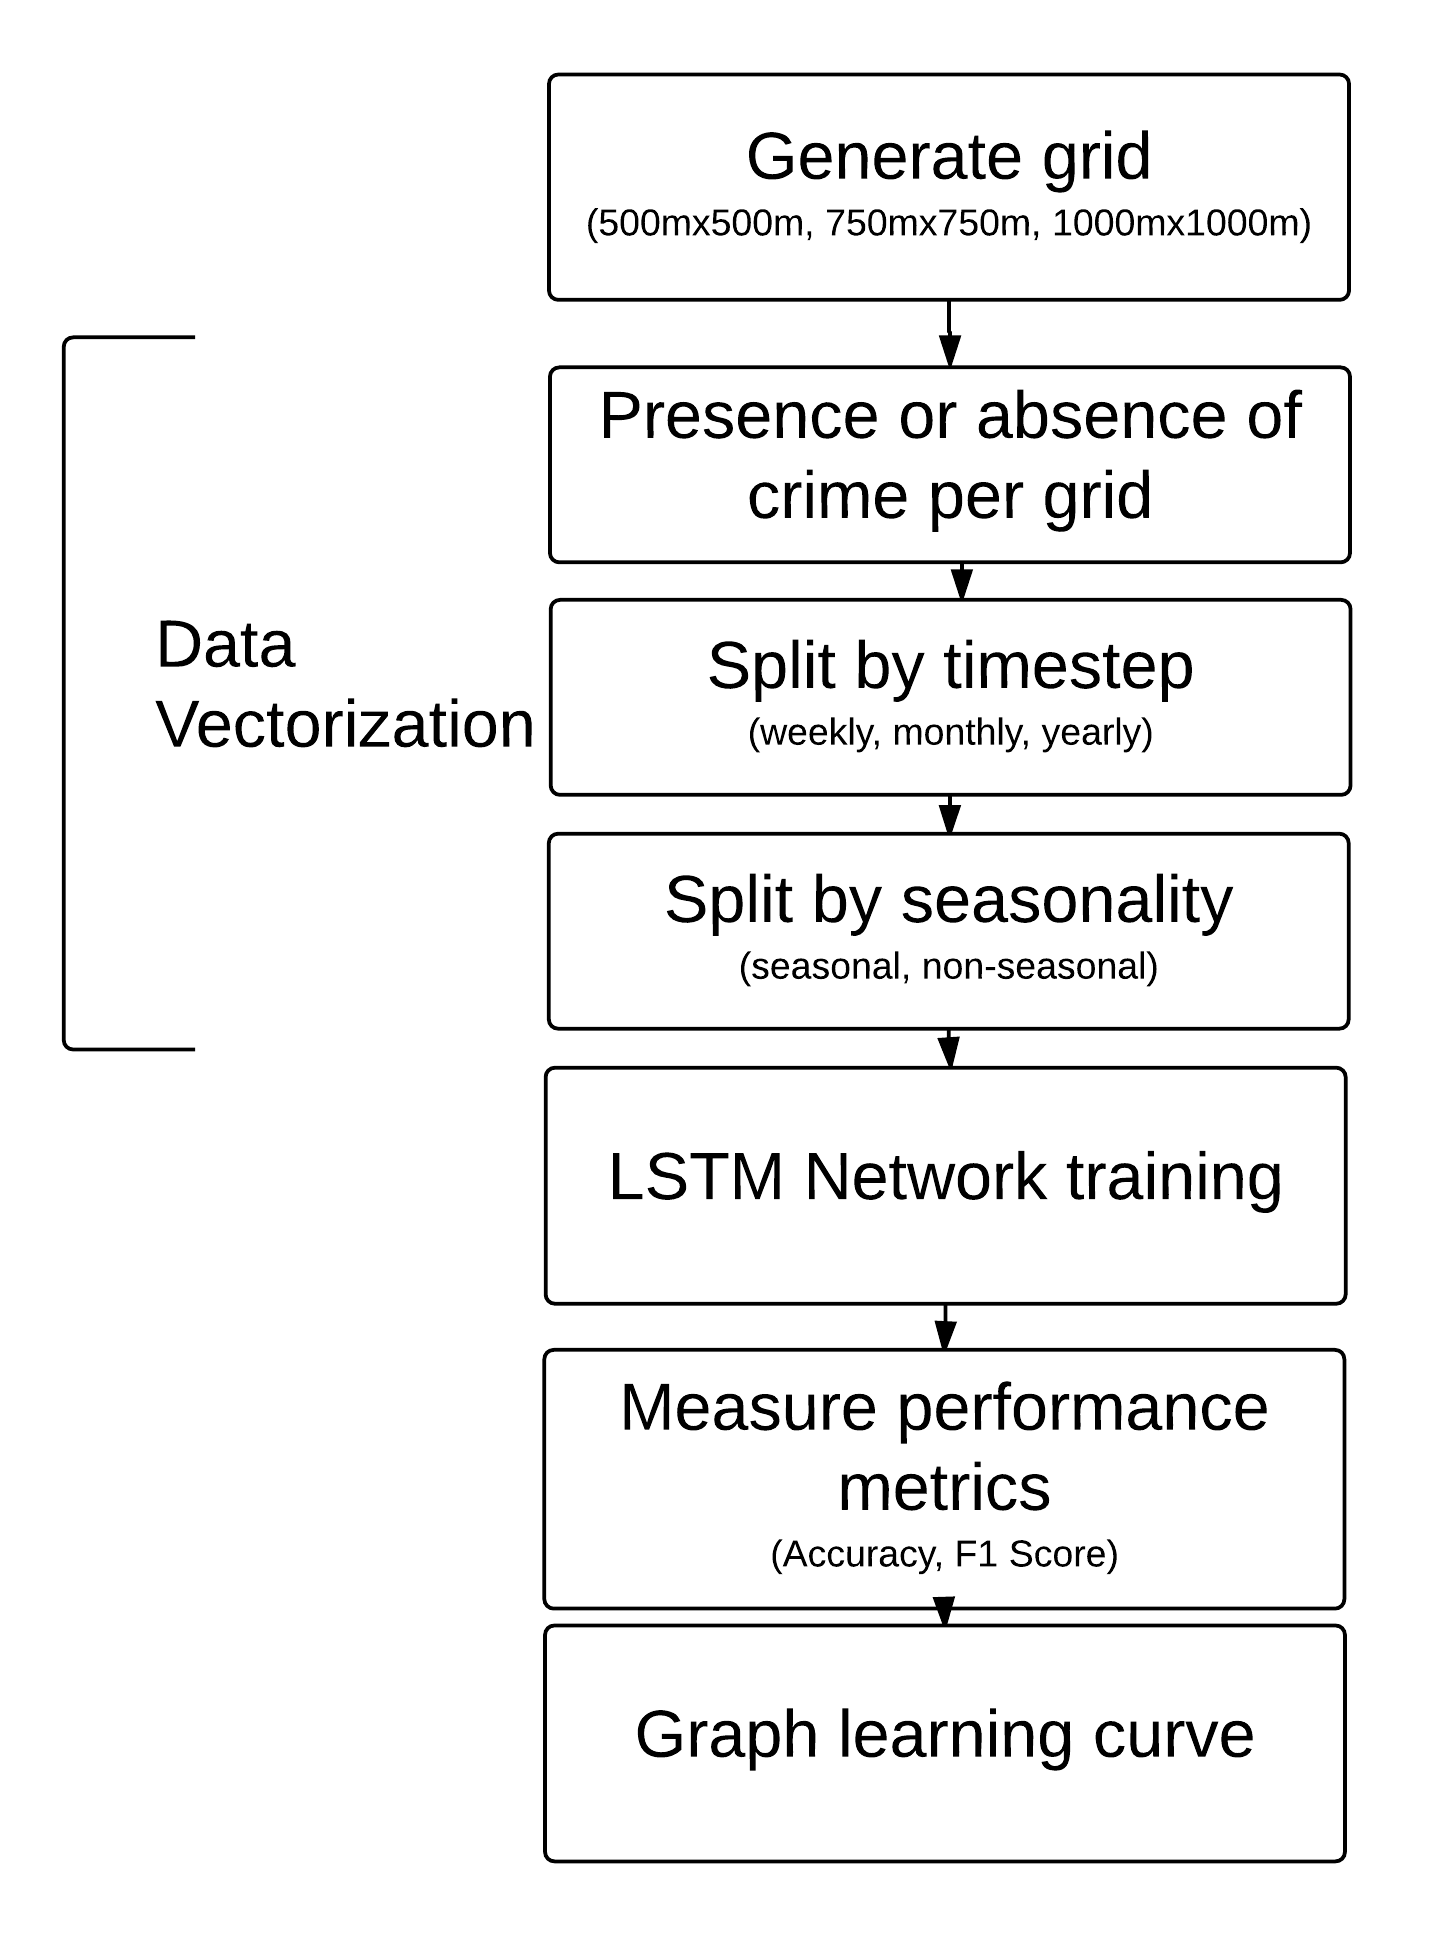
\includegraphics[width=7cm]{conceptual-framework}
    \caption{The conceptual framework of the study}
    \label{fig:conceptual-framework}
\end{figure}
Grid thematic mapping is applied to the study area, which is Chicago and grid overlay is produced. This is done for three different cell dimensions, 500mx500m, 750mx750m and 1000mx1000m. After generating the grid, data vectorization is done through different values of timestep. The different timestep values are 'monthly', 'weekly', and 'yearly'. The data vector contains values of 1 and -1 for each cell in the grid indicating the presence or absence of crime in that cell and is repeated for each month, week or year. Crime seasonality is also considered in data vectorization. Instead of getting consequent arrays of 1 and -1 for each cell for each month or week, the array is obtained for the same month or week of each year.

After processing the data, the vector is fed into an LSTM network. The input of the network is the single timestep $t$ of 1s and -1s for each cell and the target output is the values of next timestep $t+1$. The next input is from timestep $t+1$ and the target output is $t+2$ and so on. The LSTM layer contains number of nodes equal to the number of cells in the grid. After the training, the LSTM network's weight matrix should be able to approximate if the cells in the grid are crime hotspots or not.

The LSTM network's performance is measured and evaluated with accuracy and F1 score as performance metrics. Accuracy is the number of correct predictions made divided by the total made predictions. F1 score is the weighted average of the model's precision and recall \cite{scikit-learn}. Precision is the ability of the model not to classify negative examples as positive. It is defined by the equation: \( precision = tp / (tp + fp) \), where $tp$ is the true positives or the number of correct positive labels, and $fp$ is the false positives or the number of incorrect positive labels. Recall is the ability of the model to predict all positive examples. It is defined by the equation: \( recall = tp / (tp + fn) \), where $fn$ is the false negatives or the number of incorrect negative labels. Finally, F1 score is represented as the equation \(F1 = 2 * (precision * recall) / (precision + recall)\).

To understand the performance of the LSTM network, error analysis is done by generating learning curves from its training error and validation error.